% ======================= DESCRIPCIÓN DEL DATASET =====================
\section{Descripción del Dataset}
\label{sec:dataset}

\subsection{Origen}

La fuente es \textbf{GH Archive} (\url{https://www.gharchive.org}), un proyecto abierto que registra la línea de tiempo pública de GitHub a partir de su API de eventos y la publica como archivos horarios. Cada archivo contiene los eventos de una hora, uno por línea, en formato JSON comprimido con \textit{gzip}, y se descarga desde una dirección predecible:

\begin{center}
\texttt{https://data.gharchive.org/AAAA-MM-DD-H.json.gz} \qquad (\texttt{H} de 0 a 23, hora UTC)
\end{center}

El dataset cumple los cuatro requisitos del enunciado, como resume la Tabla~\ref{tab:requisitos-dataset}.

\begin{table}[H]
\centering
\caption{Cumplimiento de los requisitos de la fuente de datos}
\label{tab:requisitos-dataset}
\vspace{0.2cm}
\small
\begin{tabular}{@{}p{5.0cm}p{9.7cm}@{}}
\toprule
\textbf{Requisito} & \textbf{Cumplimiento} \\
\midrule
Naturaleza semiestructurada   & JSON con cabecera común y un \texttt{payload} cuya estructura depende del tipo de evento (16 tipos observados). \\
Al menos 50,000 registros     & 31,244,224 eventos válidos cargados; un solo día completo aporta entre 81 mil y 2.07 millones. \\
Actualización periódica       & La fuente publica un archivo nuevo cada hora; el DAG incorpora una hora por ejecución. \\
Origen y estructura documentados & Esta sección; exploración inicial en \repo{notebooks/01_exploracion_dataset.ipynb}{notebooks/01\_exploracion\_dataset.ipynb}. \\
\bottomrule
\end{tabular}
\end{table}

\subsection{Estructura de un Evento}

Todos los eventos comparten los campos de la Tabla~\ref{tab:campos}. El \textit{pipeline} conserva los campos de identificación de la cabecera y recorta el \texttt{payload} a los campos relevantes de cada tipo, lo que reduce el documento almacenado a un promedio de 263~bytes.

\begin{table}[H]
\centering
\caption{Campos de un evento de GH Archive y tratamiento en el \textit{pipeline}}
\label{tab:campos}
\vspace{0.2cm}
\small
\begin{tabular}{@{}llp{5.3cm}p{4.6cm}@{}}
\toprule
\textbf{Campo} & \textbf{Tipo} & \textbf{Descripción} & \textbf{Tratamiento} \\
\midrule
\texttt{id}          & cadena  & Identificador único del evento & Obligatorio; pasa a ser \texttt{\_id} \\
\texttt{type}        & cadena  & Tipo de evento (\texttt{PushEvent}, \texttt{PullRequestEvent}, \ldots) & Obligatorio \\
\texttt{actor}       & objeto  & Usuario que origina el evento & Se conservan \texttt{id} y \texttt{login} (obligatorio) \\
\texttt{repo}        & objeto  & Repositorio afectado & Se conservan \texttt{id} y \texttt{name} (obligatorio) \\
\texttt{org}         & objeto  & Organización dueña del repositorio & Opcional; se omite si no existe \\
\texttt{payload}     & objeto  & Detalle específico del tipo & Recortado por tipo \\
\texttt{public}      & booleano & Visibilidad del evento & Se conserva \\
\texttt{created\_at} & fecha   & Instante del evento (ISO-8601, UTC) & Obligatorio; se convierte a fecha nativa \\
\bottomrule
\end{tabular}
\end{table}

\bloque{Evento de tipo \texttt{PullRequestEvent} tal como queda almacenado en MongoDB}
\begin{lstlisting}[style=plano]
{
  "_id": "19739802706",
  "type": "PullRequestEvent",
  "actor": { "id": 231292269, "login": "sammykenny2" },
  "repo":  { "id": 1307565161, "name": "cats-inc/cats-platform" },
  "org":   { "id": 269868467, "login": "cats-inc" },
  "payload": { "action": "opened", "number": 425, "title": "", "merged": null },
  "public": true,
  "created_at": "2026-11-11T02:59:49.000Z"
}
\end{lstlisting}

\subsection{Volumen y Composición}

La Tabla~\ref{tab:volumen} resume el volumen cargado y la Tabla~\ref{tab:tipos} su composición por tipo de evento.

\begin{table}[H]
\centering
\caption{Volumen del dataset al corte del 11 de noviembre de 2026, 03:00 UTC}
\label{tab:volumen}
\vspace{0.2cm}
\small
\begin{tabular}{@{}lr@{}}
\toprule
\textbf{Métrica} & \textbf{Valor} \\
\midrule
Periodo cubierto                         & 1 oct -- 11 nov 2026 \\
Archivos horarios procesados             & 985 \\
Días con las 24 horas cargadas           & 40 \\
Tamaño de los archivos de origen (comprimidos) & 8.4 GB \\
Eventos crudos leídos                    & 31,244,816 \\
Eventos válidos cargados                 & 31,244,224 \\
Tipos de evento distintos                & 16 \\
Tamaño medio del documento en MongoDB    & 263 bytes \\
\bottomrule
\end{tabular}
\end{table}

\begin{table}[H]
\centering
\caption{Composición del dataset por tipo de evento (agregación sobre la colección \texttt{events})}
\label{tab:tipos}
\vspace{0.2cm}
\small
\begin{tabular}{@{}lrr@{}}
\toprule
\textbf{Tipo de evento} & \textbf{Eventos} & \textbf{\% del total} \\
\midrule
\texttt{PushEvent}                      & 22,369,625 & 71.60 \\
\texttt{CreateEvent}                    &  3,140,657 & 10.05 \\
\texttt{PullRequestEvent}               &  1,656,815 &  5.30 \\
\texttt{DeleteEvent}                    &  1,316,406 &  4.21 \\
\texttt{IssueCommentEvent}              &    816,179 &  2.61 \\
\texttt{IssuesEvent}                    &    677,852 &  2.17 \\
\texttt{PullRequestReviewEvent}         &    405,565 &  1.30 \\
\texttt{WatchEvent}                     &    308,395 &  0.99 \\
\texttt{PullRequestReviewCommentEvent}  &    228,823 &  0.73 \\
\texttt{ReleaseEvent}                   &    208,899 &  0.67 \\
\texttt{ForkEvent}                      &     51,700 &  0.17 \\
Otros cinco tipos                       &     63,308 &  0.20 \\
\midrule
\textbf{Total}                          & \textbf{31,244,224} & \textbf{100.00} \\
\bottomrule
\end{tabular}
\end{table}

\subsection{Actualización Incremental}

La actualización periódica no se simula: la fuente crece realmente una hora cada hora. El sistema la incorpora por dos vías que comparten el mismo código.

\begin{itemize}[leftmargin=*]
    \item \textbf{Presente (Airflow).} El DAG se ejecuta cada hora y procesa el archivo de la hora \texttt{data\_interval\_start} menos un retraso configurable (\texttt{GHARCHIVE\_LAG\_HOURS = 2}), porque GH Archive publica cada archivo con una demora de una a dos horas.
    \item \textbf{Pasado (carga histórica).} El \textit{script} \repo{scripts/backfill_days.py}{scripts/backfill\_days.py} recorre un rango de fechas configurable e invoca, hora por hora, las mismas funciones que usa el DAG. Así se cargó el periodo del 1 de octubre al 10 de noviembre.
\end{itemize}

En ambos casos la unidad de trabajo es \textbf{una hora}, y cada hora se registra en la tabla \texttt{pipeline\_runs} de Cassandra, que al corte contiene exactamente 985 filas, una por archivo procesado.

\subsection{Calidad de los Datos}
\label{subsec:calidad}

La etapa de validación aplica tres reglas: presencia de los campos obligatorios (\texttt{id}, \texttt{type}, \texttt{actor.login}, \texttt{repo.name}, \texttt{created\_at}), fecha interpretable en ISO-8601 y unicidad del identificador dentro del lote. Para verificar su efecto real, y descartar que el \textit{pipeline} estuviera eliminando datos, se realizó una auditoría independiente: un programa aparte leyó los 985 archivos crudos, les aplicó la función de validación y comparó el resultado con lo almacenado.

\begin{table}[H]
\centering
\caption{Auditoría de los 985 archivos de origen frente a lo cargado}
\label{tab:auditoria}
\vspace{0.2cm}
\small
\begin{tabular}{@{}lrr@{}}
\toprule
\textbf{Concepto} & \textbf{Eventos} & \textbf{\% del crudo} \\
\midrule
Eventos crudos leídos                               & 31,244,816 & 100.0000 \\
Rechazados por validación (\texttt{repo.name} ausente) &        190 &   0.0006 \\
Descartados por identificador duplicado             &        402 &   0.0013 \\
Líneas con JSON inválido                            &          0 &   0.0000 \\
\midrule
Eventos válidos esperados                           & 31,244,224 &  99.9981 \\
Documentos en MongoDB (\texttt{events})             & 31,244,224 &  99.9981 \\
\bottomrule
\end{tabular}
\end{table}

Tres comprobaciones adicionales cierran la auditoría: (i) el número de líneas de cada archivo intermedio coincide con los eventos válidos esperados en los 985 casos, sin una sola diferencia; (ii) ninguna hora alcanzó el tope de 200,000 eventos por corrida (el máximo observado fue 94,617), por lo que no hubo truncamiento; y (iii) el único motivo de rechazo en todo el periodo fue la ausencia del nombre del repositorio. \textbf{El \textit{pipeline} conserva el 99.998\,\% de lo que entrega la fuente.}

\subsection{Hallazgo: la Cobertura de la Fuente no es Constante}
\label{subsec:cobertura}

\paragraph{El síntoma.} El volumen de los 40 días completos varía entre 81,054 y 2,073,894 eventos: un factor de 25.6 entre días que tienen, todos, sus 24 horas cargadas. La actividad real de una plataforma como GitHub no cambia en esa proporción de un día al siguiente, y el 6 al 7 de octubre el total cae de 1.5 millones a 162 mil.

\paragraph{Lo que se descartó.} La auditoría de la Sección~\ref{subsec:calidad} elimina la hipótesis de un filtro propio. Además, la descarga copia el archivo byte a byte y su tamaño local coincide con el que reporta el servidor de GH Archive (verificado, por ejemplo, para \texttt{2026-10-01-12}: 18,566,754 bytes en ambos extremos). El dato ya llega así.

\paragraph{La causa observable.} Al desagregar por tipo de evento aparece un patrón nítido. Los eventos se comportan como \textbf{dos flujos independientes}:

\begin{itemize}[leftmargin=*]
    \item \textbf{Flujo de referencias de Git} (\texttt{PushEvent}, \texttt{CreateEvent}, \texttt{DeleteEvent}): representa el 85.9\,\% del dataset y es \textbf{intermitente}. Los tres tipos aparecen y desaparecen juntos: de los 985 archivos horarios, 505 contienen los tres y 480 no contienen ninguno; no existe un solo archivo con uno de ellos y sin los otros. El corte ocurre además dentro de la hora: en 93 archivos el flujo está presente solo durante parte de los minutos.
    \item \textbf{Flujo de colaboración} (\textit{pull requests}, \textit{issues}, comentarios, revisiones, estrellas, \textit{releases}): es \textbf{estable} durante todo el periodo, entre 59,870 y 246,785 eventos diarios.
\end{itemize}

\begin{figure}[H]
    \centering
    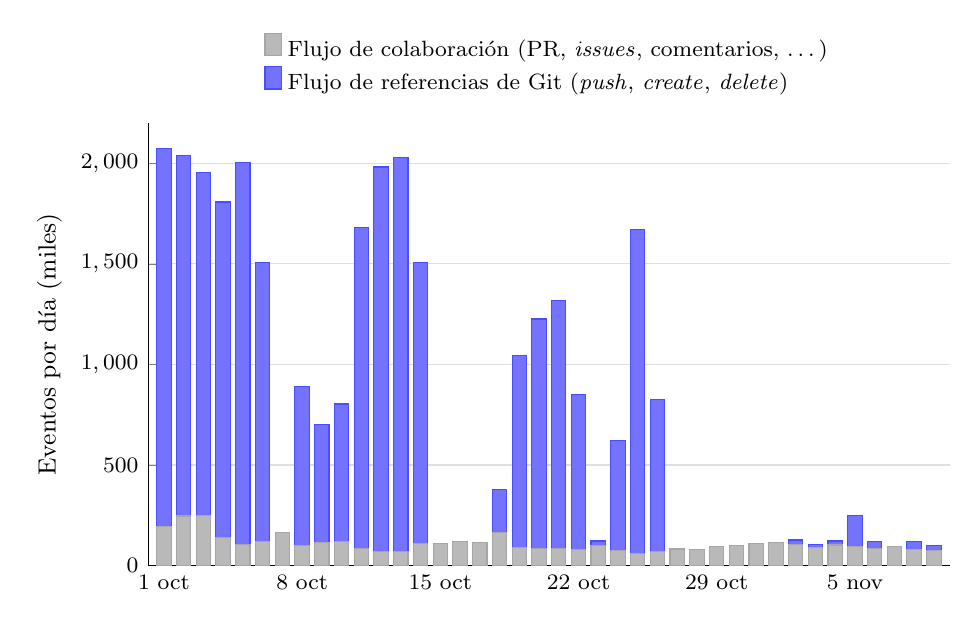
\begin{tikzpicture}
    \begin{axis}[
        ybar stacked, bar width=5.2pt,
        width=0.97\textwidth, height=7.2cm,
        ymin=0, ymax=2200,
        xmin=-0.8, xmax=39.8,
        ylabel={Eventos por día (miles)},
        ylabel style={font=\small},
        tick label style={font=\footnotesize},
        xtick={0,7,14,21,28,35},
        xticklabels={1 oct, 8 oct, 15 oct, 22 oct, 29 oct, 5 nov},
        ymajorgrids, grid style={gray!25},
        axis lines*=left,
        legend style={font=\footnotesize, at={(0.5,1.04)}, anchor=south, draw=none, legend columns=1, legend cell align=left},
        scaled y ticks=false,
        yticklabel={\pgfmathprintnumber[fixed, 1000 sep={,}]{\tick}},
    ]
    \addplot[fill=gray!55, draw=gray!70] coordinates {(0,193.5) (1,246.2) (2,246.8) (3,140.7) (4,102.4) (5,120.9) (6,162.5) (7,99.8) (8,114.6) (9,118.0) (10,83.3) (11,71.6) (12,69.5) (13,109.4) (14,111.2) (15,121.4) (16,114.8) (17,163.7) (18,90.9) (19,83.1) (20,82.5) (21,77.8) (22,100.2) (23,73.7) (24,59.9) (25,68.8) (26,82.1) (27,81.1) (28,94.1) (29,98.7) (30,107.7) (31,115.3) (32,104.1) (33,90.5) (34,102.2) (35,95.7) (36,86.1) (37,94.4) (38,79.2) (39,74.8)};
    \addplot[fill=blue!55, draw=blue!70] coordinates {(0,1880.4) (1,1794.8) (2,1707.9) (3,1667.1) (4,1903.2) (5,1384.8) (6,0.0) (7,791.4) (8,587.0) (9,685.3) (10,1597.6) (11,1910.4) (12,1960.3) (13,1396.3) (14,0.0) (15,0.0) (16,0.0) (17,213.5) (18,951.8) (19,1142.6) (20,1237.0) (21,772.7) (22,21.7) (23,546.1) (24,1610.5) (25,755.6) (26,0.0) (27,0.0) (28,0.0) (29,0.0) (30,0.0) (31,0.0) (32,22.9) (33,15.2) (34,19.6) (35,151.1) (36,35.0) (37,0.0) (38,42.2) (39,22.9)};
    \legend{Flujo de colaboración (PR{,} \textit{issues}{,} comentarios{,} \ldots), Flujo de referencias de Git (\textit{push}{,} \textit{create}{,} \textit{delete})}
    \end{axis}
    \end{tikzpicture}
    \caption{Eventos por día en los 40 días completos, separados en los dos flujos (conteo sobre los archivos de origen). El flujo de colaboración (gris) es estable; el de referencias de Git (azul) aparece y desaparece en bloque.}
    \label{fig:cobertura}
\end{figure}

\begin{table}[H]
\centering
\caption{Los 40 días completos según la presencia de \texttt{PushEvent} en sus archivos horarios}
\label{tab:cobertura}
\vspace{0.2cm}
\small
\begin{tabular}{@{}p{5.2cm}rrp{4.6cm}@{}}
\toprule
\textbf{Situación del día} & \textbf{Días} & \textbf{Media de eventos} & \textbf{Fechas} \\
\midrule
\textit{Push} en las 24 horas        & 12 & 1,736,165 & 1--5, 11--13, 19--21 y 25 oct \\
\textit{Push} en parte de las horas  & 17 &   \multicolumn{1}{c}{--} & 6, 8--10, 14, 18, 22--24, 26 oct; 2--6, 8, 9 nov \\
Sin ningún \textit{push}             & 11 &   107,570 & 7, 15--17, 27--31 oct; 1 y 7 nov \\
\bottomrule
\end{tabular}
\end{table}

La comparación es contundente: los días con el flujo de Git completo promedian 1.74 millones de eventos y los días sin él, 108 mil; en cambio, el flujo de colaboración varía en un factor de 4.1 frente al 25.6 del total. Una muestra de la misma hora (12:00 UTC) en tres fechas lo confirma a nivel de archivo (Tabla~\ref{tab:muestra-horas}).

\begin{table}[H]
\centering
\caption{Contenido del archivo de las 12:00 UTC en tres fechas}
\label{tab:muestra-horas}
\vspace{0.2cm}
\footnotesize
\begin{tabular}{@{}lrrrr@{}}
\toprule
\textbf{Archivo} & \textbf{Eventos} & \texttt{PushEvent} & \texttt{PullRequestEvent} & \texttt{IssuesEvent} \\
\midrule
\texttt{2026-10-01-12} & 92,323 & 70,908 & 2,608 & 888 \\
\texttt{2026-10-28-12} &  3,840 &      0 & 1,346 & 686 \\
\texttt{2026-11-05-12} & 12,814 &  7,132 & 1,633 & 600 \\
\bottomrule
\end{tabular}
\end{table}

\paragraph{Contraste con fuentes externas.} El comportamiento coincide con un reporte abierto en el repositorio del propio GH Archive\footnote{\textit{Hourly archives dropped to \textasciitilde 3k events per hour since 2026-10-27}, \url{https://github.com/igrigorik/gharchive.org/issues/326}.}, que documenta la misma caída y reporta para el archivo \texttt{2026-10-01-12} exactamente los 92,323 eventos medidos aquí. Ese reporte atribuye el problema al colector de GH Archive, que según sus autores no alcanza a recorrer todas las páginas de la API de eventos de GitHub. Esa explicación es de terceros y este proyecto no puede verificarla; lo que sí queda verificado con los datos propios es el patrón de dos flujos y su calendario.

\paragraph{Implicaciones para el análisis.} El hallazgo no invalida los indicadores, pero delimita qué puede afirmarse con ellos:

\begin{enumerate}[leftmargin=*]
    \item El volumen total diario mide, ante todo, \textbf{la cobertura del colector}, no la actividad de GitHub. Las variaciones del KPI~1 y del KPI~2 entre un día con \textit{push} y otro sin él son un artefacto de la fuente.
    \item Los indicadores que no dependen del flujo de Git siguen siendo comparables entre días. La tasa de fusión de \textit{pull requests} (KPI~4) se mantiene entre 88.8\,\% y 94.7\,\% en todo el periodo precisamente porque se apoya en el flujo estable.
    \item El \textit{dashboard} advierte esta limitación en las lecturas de sus gráficos y en su pestaña de metodología, en lugar de presentar las variaciones como tendencias reales.
\end{enumerate}
